\begin{figure}
  \centering
  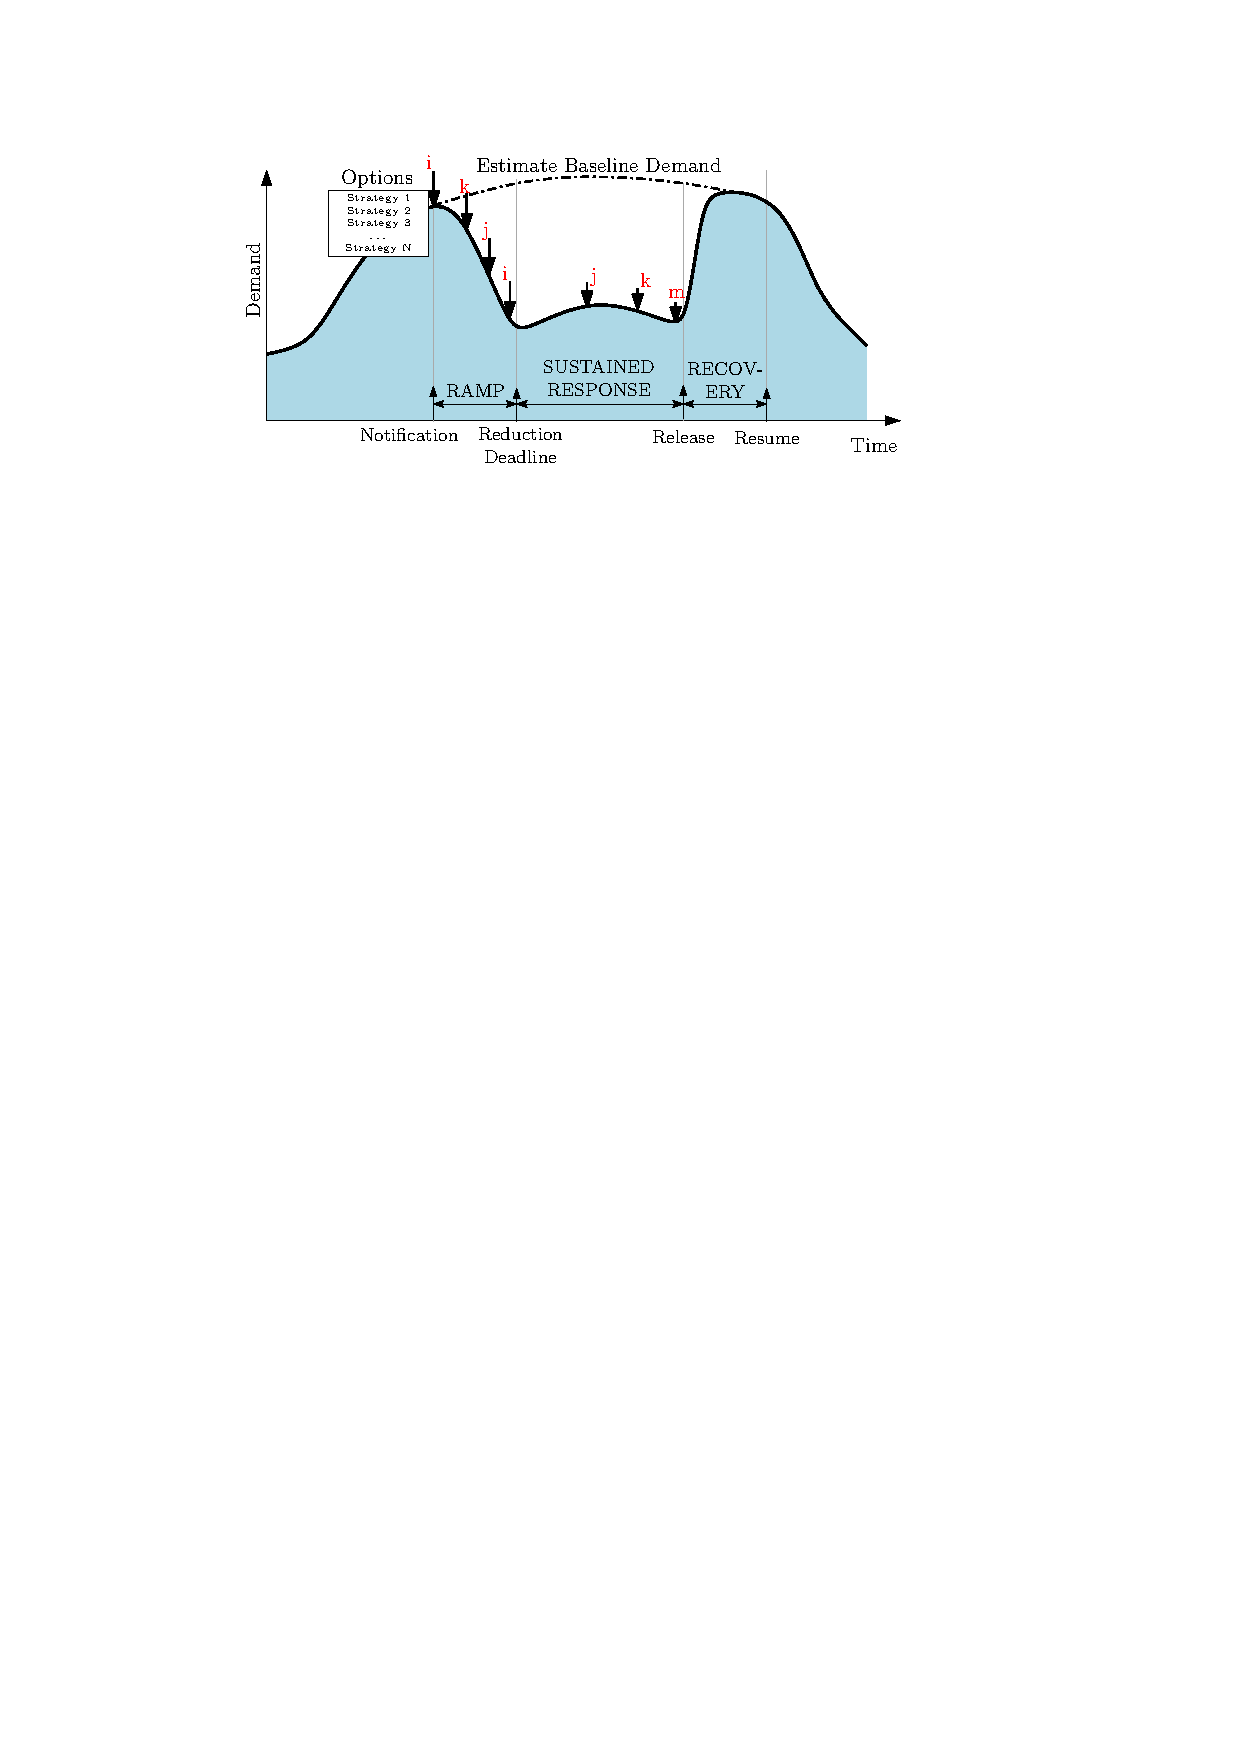
\includegraphics[width=0.75\columnwidth]{figs/problem_description}
  \caption{Example of a demand response timeline.}
  \label{fig:baseline}
\end{figure}

The timeline of a DR event is shown in Fig.~\ref{fig:baseline}.
%An \emph{event notification} is issued by the utility/CSP, at the notification time ($\sim$30mins).
%The time by which the reduction must be achieved, is the \emph{reduction deadline}.
%The main period during which the demand needs to be curtailed is the \emph{sustained response period} (1$\sim$6hrs).
%The end of the response period is when the main curtailment is released. 
%The normal operation is gradually resumed during the \emph{recovery period}.
%The DR event ends at the end of the recovery period.
The key to answering the question of what actions to take to achieve a significant DR curtailment upon receiving a notification, lies in making accurate predictions about the power consumption response of the building. 
Specifically, it involves solving the three challenging problems of end-user demand response, which are described next.


\subsection{DR baseline prediction}
\label{sec:baselining}
The DR baseline is an estimate of the electricity that would have been consumed by a customer in the absence of a demand response event (as shown in Fig.~\ref{fig:baseline}) 
The measurement and verification of the demand response baseline is the most critical component of any DR program since the amount of DR curtailment, and any associated financial reward can only be determined with respect to the baseline estimate.
The goal is to learn a predictive model $f$ which relates the baseline power consumption estimate $\mathcal{P}_{\mathrm{base}}$ to the forecast of the weather conditions $\mathcal{W}$ and building schedule $\mathcal{S}$ for the duration of the DR-event, i.e. $\mathcal{P}_{\mathrm{base}} = f(\mathcal{W},\mathcal{S})$.


\subsection{DR strategy evaluation}
\label{sec:eval}
%Most DR today is manual and conducted using fixed rules and pre-determined curtailment strategies based on recommended guidelines, experience and best practices. 
During a DR event, the building's facilities manager must choose a single strategy among several pre-determined strategies to achieve the required power curtailment. 
Each strategy includes adjusting several control knobs such as temperature set-points, lighting levels and temporarily switching off equipment and plug loads to different levels across different time intervals. 
As only one strategy can be used at a time, the question then is, \emph{how to choose the DR strategy from a pre-determined set of strategies which leads to the largest load curtailment?}

Instead of predicting the baseline power consumption $\mathcal{P}_{\mathrm{base}}$, in this case we want the ability to predict the actual response of the building $\mathcal{P}$ due to any given strategy.
For example, in Fig.~\ref{fig:baseline}, there are $N$ different strategies available to choose from. 
DR-Advisor predicts the power consumption of the building due to each strategy and chooses the DR strategy $(1,\dots, N)$ which leads to the largest load curtailment.
The resulting strategy could be a combination of switching between the available set of strategies.

\subsection{DR strategy synthesis}
\label{sec:synthesis}
Instead of choosing a DR strategy from a pre-determined set of strategies, a harder challenge is to synthesize new DR strategies and obtain optimal operating points for the different control variables.
We can cast this problem as the following optimization over the set of control variables $\mathbb{X}_c$
%\begin{equation}
%\begin{aligned}
%& \underset{\mathbb{X}_c}{\text{minimize}}
%& & f(\hat{Y_{kW}}) \\
%& \text{subject to}
%& & \hat{Y_{kW}} = h(\mathbb{X}_c) \\
%& & & \mathbb{X}_c \in \mathbb{X}_{safe}
%\end{aligned}
%\label{eq:linear_program}
%\end{equation}
\begin{align}
\begin{aligned}
\text{minimize } \ \ \ & \ \mathit{g} \left( \mathbb{Y}, \mathbb{X}_c  \right) \\ 
\text{subject to } \ \ \ & \mathbb{Y} = h \left( \mathbb{X}_c \right), \\ 
\ \ \ & \ \mathbb{X}_c \in \mathbb{X}_{\mathrm{des}},
  \end{aligned}
  \label{eq:linear_program}
\end{align}
where we want to minimize the predicted power response of the building $\mathbb{Y}:=\mathcal{P}$, subject to a predictive model which relates the response to the control variables and subject to the constraints on the control variables.
Unlike rule-based DR, which does not account for building state and external factors, in DR synthesis the optimal control actions are derived based on the current state of the building, forecast of outside weather and electricity prices.